% these figures are not mentioned anywhere, use \ref{fig:rand1} to reference them
\begin{figure}
\centering
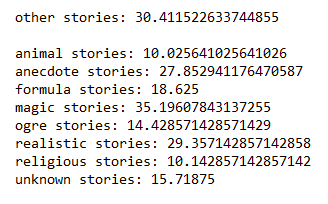
\includegraphics[]{random/directspeechtext.PNG}
% is it average? then write it
\caption{The average number of direct speeches per text in the ATU-index groups.}
% label for every figure must be unique!
\label{fig:rand1}
\end{figure}

\begin{figure}
\centering
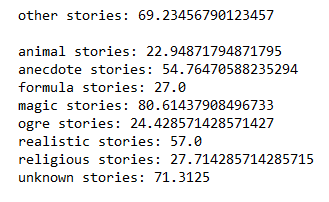
\includegraphics[]{random/sentencestext.PNG}
\caption{The average amount of sentences per text in the ATU-index groups.}
\label{fig:rand2}
\end{figure}

\begin{figure}
\centering
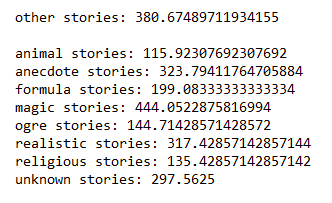
\includegraphics[]{random/specialsignstext.PNG}
\caption{The average number special signs per text in the ATU-index groups.}
\label{fig:rand3}
\end{figure}

\begin{figure}
\centering
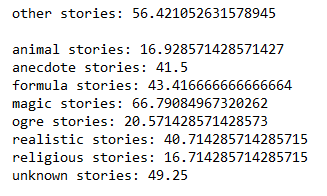
\includegraphics[]{random/propernames_text_.PNG}
\caption{The average number proper names per text in the ATU-index groups.}
\label{fig:rand4}
\end{figure}

\begin{figure}
\centering
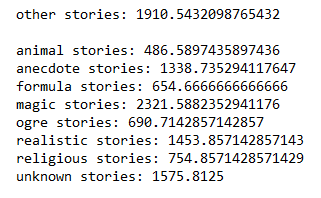
\includegraphics[]{random/wordstext.PNG}
\caption{The average amount of words per text in the ATU-index groups.}
\label{fig:rand5}
\end{figure}

\begin{figure}
\centering
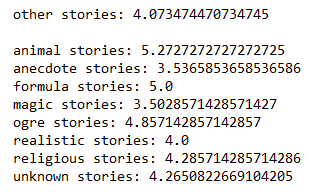
\includegraphics[]{random/wordstitle.PNG}
\caption{The average amount of words per title in the ATU-index groups.}
\label{fig:rand6}
\end{figure}
